% ============================================================================
% Poster A0 - "Pressure Measurement in Confined Systems of Self-Propelled
% Particles via FSR Sensors" -- Integral (Perimeter) Configuration.
%
% Layout (matches the user-provided wireframe mockup):
%   Header: title + subtitle + authors + affiliations + emails + logos.
%   Row 1: Abstract (span=6, full width).
%   Row 2: Experimental Setup & Acquisition Chain (span=6, one header,
%          THREE internal sub-columns via a tabular: Setup | Acquisition
%          Chain (circuit schematic) | Analysis Pipeline).
%   Row 3: dG Distributions & Skewness (span=3) | Dynamics & Survival (span=3).
%   Row 4: Conclusions, Acknowledgements & References (span=6, one header,
%          THREE internal sub-columns: Conclusions & Next Steps |
%          Acknowledgements | References).
%
% IMPORTANT (baposter mechanics, learned the hard way -- keep these notes
% when editing further):
%  1) bottomaligned=X needs box X to already be typeset earlier IN THE
%     SOURCE (pgf resolves that anchor in source order, not by column/
%     visual position).
%  2) A box left with NO "below"/"aligned" key defaults to row=0, i.e.
%     flush under the header. Only Abstract (the very first box) does
%     that here; every other box uses an explicit below=<name>.
%  3) bottomaligned only overrides the box's FRAME height -- it does NOT
%     reflow or shrink content. If the dependent box's own content is
%     taller than the reference, it overflows past its own border --
%     silently, with no compile warning.
%  4) headerheight / boxheaderheight / colspacing / boxpadding are all in
%     "em" units that get amplified by 1/fontscale (here 1/0.292 ~= 3.4x)
%     when baposter blows the internally-typeset page up to real A0 size.
%     A tiny change in the source can move ~10% of the page's real height.
%     IMPORTANT LESSON FROM THIS SESSION: boxheaderheight was squeezed too
%     far (down to 0.46em) while chasing overflow -- the box header TEXT
%     (e.g. "EXPERIMENTAL SETUP...") no longer fit vertically inside its
%     own header bar and got silently clipped at the top, same failure
%     mode as note 3 but for the header instead of the body. 0.65em is the
%     floor that has been visually verified clean; do not go below it.
%  5) baposter never reflows to fit the physical page: if total content
%     height exceeds the A0 page, the excess is clipped invisibly, no
%     error, no second page. ALWAYS verify by rendering + cropping the
%     bottom edge of the PDF, never trust "no LaTeX errors" alone.
%  6) A box that contains raw (non-circuitikz) TikZ drawn in absolute cm
%     units does NOT auto-scale to the column width the way width=\linewidth
%     images do -- wrap it in \resizebox{<fraction>\linewidth}{!}{...} same
%     as circuitikz, or it prints at a fixed physical cm size that can look
%     tiny (wide box) or overflow (narrow box). A WIDE/SHORT drawing (like
%     the op-amp circuit below: opamp + feedback loop + MCU box, all in a
%     row) forced into a NARROW column still comes out reasonably short
%     once resized, because resizebox preserves aspect ratio -- don't
%     assume "wide source drawing" automatically means "tall once narrow".
%  7) A single posterbox can hold an internal N-column layout with a
%     tabular using p{width} columns (p{} columns top-align by default,
%     like \parbox[t]) -- this is how "Setup & Acquisition Chain" and
%     "Conclusions, Acknowledgements & References" each pack 3 sub-panels
%     under one shared header, matching the mockup.
%  8) Vertical spacing is kept to a SMALL, CONSISTENT set of values
%     (\smallskip / \medskip, both font-relative) instead of a pile of
%     ad-hoc \vspace{0.05em}/\vspace{0.35em}/etc scattered per edit --
%     the latter is what produced visibly inconsistent gaps across boxes
%     in an earlier iteration of this file.
% ============================================================================
\documentclass[portrait,a0paper,fontscale=0.292]{baposter}

\usepackage{amsmath,amsfonts,amssymb}
\usepackage{graphicx}
\usepackage{grffile} % allows filenames with spaces, e.g. "Skewness vs deltaT.pdf"
\usepackage{multicol} % defines \raggedcolumns, used below
\usepackage[utf8]{inputenc}
\usepackage[T1]{fontenc}
\usepackage{xcolor}
\usepackage{enumitem}
\usepackage{array}
\usepackage{tikz}
\usepackage{circuitikz}
\usetikzlibrary{arrows.meta,positioning,calc,shapes.geometric}
\ctikzset{bipoles/thickness=1.1}

% --- "SAGE GREEN" PALETTE -- CHANGE COLORS HERE -------------------------
\definecolor{sageDark}{HTML}{3F5344}   % borders, header
\definecolor{sageMid}{HTML}{5C7A57}    % header (gradient)
\definecolor{sagePale}{HTML}{EDF2E9}   % box fill
\definecolor{canvasBg}{HTML}{AFC6A0}   % page background -- CHANGE GRADIENT STRENGTH HERE (was E2E9DC, too pale to read as a gradient)
\definecolor{ink}{HTML}{222B20}        % body text
\definecolor{scopeBorder}{HTML}{3F5344}
\definecolor{scopeBg}{HTML}{E7EFE1}

% Trace colors (must match the exported PDFs) -- DO NOT CHANGE.
\definecolor{cVacio}{HTML}{475569}   % Empty/0 bots -- Slate Gray
\definecolor{cN25}{HTML}{0284C7}     % 25 bots -- Cerulean Blue
\definecolor{cN26}{HTML}{D97706}     % 26 bots -- Amber
\definecolor{cN27}{HTML}{BE123C}     % 27 bots -- Crimson
% Pale tints of the same 4 colors, used as light backgrounds behind the
% histogram panels (Row 3, left box) -- CHANGE TINT STRENGTH HERE (18%).
\colorlet{cVacioPale}{cVacio!18!white}
\colorlet{cN25Pale}{cN25!18!white}
\colorlet{cN26Pale}{cN26!18!white}
\colorlet{cN27Pale}{cN27!18!white}

\setlength{\fboxsep}{2.2pt}

% Color Legend helpers: a TikZ-drawn swatch (not \rule) next to a bold label.
% --- CHANGE SWATCH SIZE HERE (0.34 x 0.34 cm) ---
\newcommand{\swatch}[1]{\tikz[baseline=-0.5ex]{\filldraw[fill=#1,draw=black!45,line width=0.3pt] (0,0) rectangle (0.34,0.34);}}
\newcommand{\legendrow}[2]{\swatch{#1}\ \textbf{#2}}
% Small rounded "badge" tag, e.g. \badge{4 densities}
\newcommand{\badge}[1]{\tikz[baseline=-0.5ex]{\node[draw=sageDark,thick,fill=sagePale,rounded corners=2pt,inner sep=3pt,font=\footnotesize]{#1};}}

\begin{document}
\color{ink}
\raggedcolumns

\begin{poster}{
  background=shadetb, bgColorOne=white, bgColorTwo=canvasBg,
  headerheight=0.092\textheight, % --- CHANGE HEADER HEIGHT HERE (Large title wraps to 2 lines + subtitle + authors + emails) ---
  columns=6,                     % 6-column grid (baposter's maximum)
  colspacing=0.4em,              % --- CHANGE COLUMN/ROW SPACING HERE (see note 4: amplified ~3.4x on the real page) ---
  headershade=plain, headershape=roundedright, textborder=roundedleft,
  linewidth=1.6pt, headerborder=closed,
  boxpadding=0.4em, boxheaderheight=1.3em, % --- CHANGE INNER MARGIN HERE (0.65em clipped header text; 1.3em gives titles visible breathing room, see note 4) ---
  eyecatcher=true, grid=false,
  borderColor=sageDark, headerColorOne=sageDark, headerColorTwo=sageMid,
  headerFontColor=white, boxColorOne=white, boxColorTwo=sagePale,
  }
  {\raisebox{-0.5\height}{
\includegraphics[height=0.95cm]{figures/logoITBA}}}
  {\textsc{\textbf{\Large Medición de presión en sistemas de partículas autopropulsadas confinadas mediante sensores FSR en configuración integral y distribuida}}}
  {\vspace{0.15em}{\normalsize Dylan Frigerio$^{1}$ and Germ\'an Patterson$^{1,2}$ -- $^{1}$ITBA \ $^{2}$CONICET\\[0.08em]
   \footnotesize\texttt{dyfrigerio@itba.edu.ar, gpatterson@itba.edu.ar}}}
  {\raisebox{-0.5\height}{
\includegraphics[height=0.95cm]{figures/logoCONICET}}}

%% ===========================================================================
%% ROW 1 -- Abstract, full width. Trimmed to 2 tight paragraphs (was 3,
%% ran too long) -- motivation+gap, then device+payoff.
%% ===========================================================================
\begin{posterbox}[name=abstract,column=0,height=auto,span=6]{{Abstract}}
\small
La materia activa se encuentra inherentemente fuera del equilibrio termodinámico, lo que implica que magnitudes fundamentales como la presión mecánica no necesariamente se comportan como en los sistemas clásicos. En particular, se ha demostrado que la presión puede depender de la geometría del contenedor y no obedecer a una ecuación de estado convencional [1,2], lo que ha abierto un debate actual sobre si es posible formular una descripción termodinámica análoga para estos sistemas. En este contexto, el flujo intermitente de partículas autopropulsadas a través de aberturas angostas exhibe atascos cuya duración y resolución están íntimamente ligadas a la presión acumulada en el sistema [3,4]. Sin embargo, la mayoría de los estudios experimentales han estimado la presión de forma indirecta a través de la deformación de estructuras flexibles [2] o mediante sensores puntuales que brindan una medición integral de la fuerza [4].

En este trabajo presentamos el desarrollo de un sensor de presión de bajo costo basado en una cinta de sensores resistivos de fuerza (FSR) para medir la presión ejercida por un sistema de agentes autopropulsados (Kilobots) confinados en un recinto circular. El dispositivo se implementa en dos configuraciones: (i) una cinta única que rodea todo el perímetro interior del recinto, proporcionando una medición integral de la presión total ejercida sobre las paredes; y (ii) múltiples cintas más cortas que permiten analizar la distribución espacial de la presión a lo largo del contenedor. El sistema de adquisición, controlado por una placa Arduino, registra las señales de los sensores y nos permite correlacionar la dinámica colectiva (formación de clusters, flujo y atascos) con la presión ejercida sobre el contenedor.

El objetivo es variar la densidad de Kilobots en el recinto para explorar regímenes de flujo libre hasta congestión, midiendo cómo la presión cambia en función de la densidad y la dinámica colectiva. La configuración distribuida nos permitirá identificar inhomogeneidades en la distribución de fuerzas asociadas a la formación de arcos o aglomeraciones contra regiones específicas de la pared, información que se pierde en una medición integral. Este desarrollo ofrece una herramienta versátil y de bajo costo para estudiar sistemáticamente la relación entre presión local, estructura colectiva y dinámica de atascos en materia activa confinada.
\end{posterbox}

%% ===========================================================================
%% ROW 2 -- Experimental Setup & Acquisition Chain: ONE header, three
%% internal sub-columns packed via a tabular (see note 7). Acquisition
%% Chain column reverted to the op-amp circuitikz schematic (was a plain
%% block flowchart -- user asked for the actual circuit back).
%% ===========================================================================
\begin{posterbox}[name=setupacq,column=0,below=abstract,height=auto,span=6]{{Experimental Setup \& Acquisition Chain}}
\setlength{\tabcolsep}{0pt}
\small
\begin{tabular}{@{}p{0.315\linewidth}@{\hspace{0.02\linewidth}}p{0.315\linewidth}@{\hspace{0.02\linewidth}}p{0.315\linewidth}@{}}
% --- Column 1: Setup ---
{\bf Setup}\par\smallskip
\begin{center}
\resizebox{0.48\linewidth}{!}{%
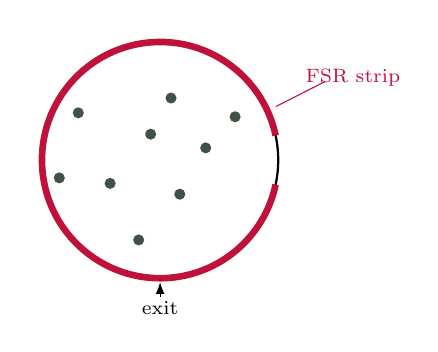
\begin{tikzpicture}
  \draw[thick] (0,0) circle (1.5cm);
  \draw[cN27, line width=2.4pt] (12:1.5cm) arc (12:348:1.5cm);
  \foreach \a/\r in {30/1.1,80/0.8,150/1.2,205/0.7,255/1.05,300/0.5,15/0.6,190/1.3,110/0.35} {
     \fill[sageDark] (\a:\r cm) circle (2.0pt);
  }
  \node[align=center, font=\scriptsize] at (0,-1.88) {exit};
  \draw[-{Latex[length=1.5mm]}, thin] (0,-1.74) -- (0,-1.55);
  \node[align=left, font=\scriptsize, cN27] at (2.45,1.05) {FSR strip};
  \draw[thin, cN27] (2.1,1.0) -- (1.47,0.68);
\end{tikzpicture}%
}
\end{center}
\smallskip
{\footnotesize\badge{4 densities}\,\badge{30 min/run}\,\badge{50 ms grid}\,\badge{10-bit ADC}}
\medskip

{\footnotesize
\begin{itemize}[itemsep=1.5pt,topsep=1pt,leftmargin=1em]
\item Circular arena, variable Kilobot density.
\item This poster: \textbf{integral} configuration only -- 1 FSR strip, full perimeter $\to$ total wall force.
\item Densities: $\varnothing$, $N=25,26,27$ (30\,min each).
\end{itemize}}
&
% --- Column 2: Acquisition Chain -- circuit schematic (as before: FSR as
% a variable resistor into an inverting transimpedance stage, feeding an
% MCU/ADC block over UART). ---
{\bf Acquisition Chain}\par\smallskip
\begin{center}
\resizebox{0.98\linewidth}{!}{%
\begin{circuitikz}[american voltages, scale=1.2, every node/.append style={font=\LARGE}, color=sageDark]
  \node[op amp] (opamp) at (3.4,0) {};
  \draw (opamp.-) -- ++(-0.7,0) coordinate(sj)
        to[vR, l=$R_{FSR}$, *-*] ++(-2.0,0) coordinate(fsrleft);
  \draw (fsrleft) -- ++(0,-0.35) coordinate(battop);
  \draw (battop) to[battery1, l_={$V_{exc}$}] ++(0,-1.15) node[ground]{};
  \draw (opamp.+) -- ++(-0.5,0) -- ++(0,-0.7) node[ground]{};
  \coordinate (fbtop) at ($(opamp.out)+(0,1.1)$);
  \coordinate (fbleft) at (sj |- fbtop);
  \draw (sj) -- (fbleft);
  \draw (fbleft) to[R, l={$R_f$}] (fbtop);
  \draw (fbtop) -- (opamp.out);
  \node[draw=sageDark, thick, fill=sagePale, minimum width=2.6cm, minimum height=2.0cm, inner sep=5pt, align=center]
    (mcu) at ($(opamp.out)+(2.1,0)$) {\Large\textbf{MCU}\\[3pt] \large 10-bit ADC\\ Averaging ($N{=}10$)};
  \draw[-{Latex[length=2mm]}] (opamp.out) -- (mcu.west);
  \draw[-{Latex[length=2.2mm]}, thick] (mcu.east) -- ++(1.0,0) node[right, align=left] {\textbf{UART}\\[-1pt] 115200 bd};
  \fill (sj) circle(1.6pt);
\end{circuitikz}%
}
\end{center}
\medskip

{\footnotesize An inverting transimpedance stage converts $R_{FSR}$ into $V_{\text{out}} = -V_{exc}\,R_f/R_{FSR}$; 
	
	The MCU digitizes and averages $N{=}10$ raw samples before logging.}
\smallskip
\begin{center}\footnotesize $G\,[\mu\text{S}] = 1/R_{FSR} \propto \text{ADC}_{\text{raw}}$\end{center}
&
% --- Column 3: Analysis Pipeline ---
{\bf Analysis Pipeline}\par\smallskip
{\footnotesize
\begin{enumerate}[itemsep=3pt,topsep=2pt,leftmargin=1.3em]
\item Resample $G(t)$ to a uniform 50\,ms grid.
\item $\delta G(t) = G(t) - G(t-\delta t)$ for a window $\delta t$.
\item Sweep $\delta t$ (50\,ms--15\,s) $\to$ skewness of $\delta G$.
\item Empirical survival function $P(G\ge g)$.
\end{enumerate}}
\medskip

{\scriptsize\itshape Same 4-condition color code and legend order in every figure: $\varnothing$ / $N{=}25$ / $N{=}26$ / $N{=}27$.}
\\
\end{tabular}
\end{posterbox}

%% ===========================================================================
%% ROW 3 -- dG Distributions & Skewness (reference box, height=auto) |
%% Dynamics & Survival (bottomaligned=distributions, written right after).
%% ===========================================================================
\begin{posterbox}[name=distributions,column=0,below=setupacq,height=auto,span=3]{{Distributions \& Skewness}}
\begin{center}
\begin{minipage}[t]{0.47\linewidth}\centering
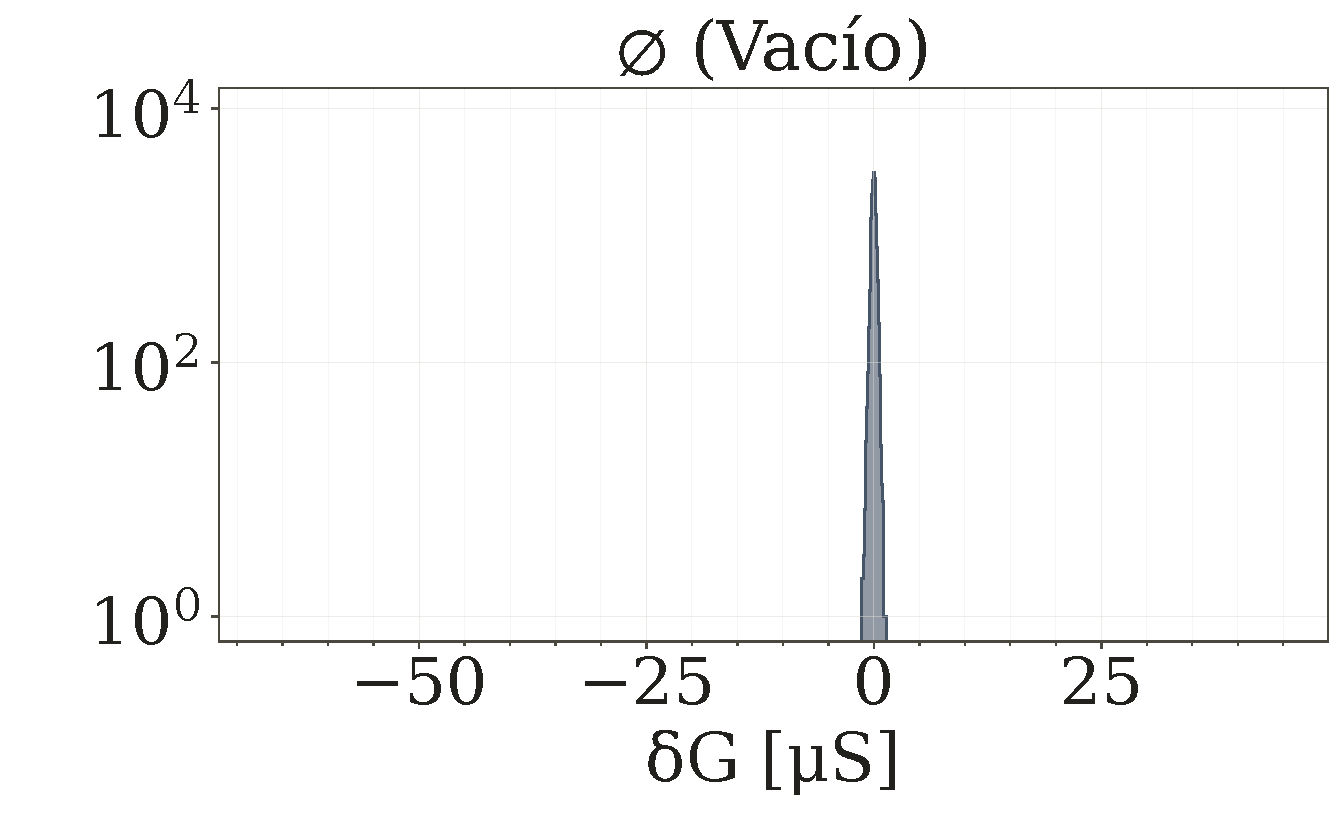
\includegraphics[width=0.68\linewidth]{figures/Null_Histogram.pdf}\\[1pt]{\footnotesize $\varnothing$ (Empty)}
\end{minipage}%
\hfill
\begin{minipage}[t]{0.47\linewidth}\centering
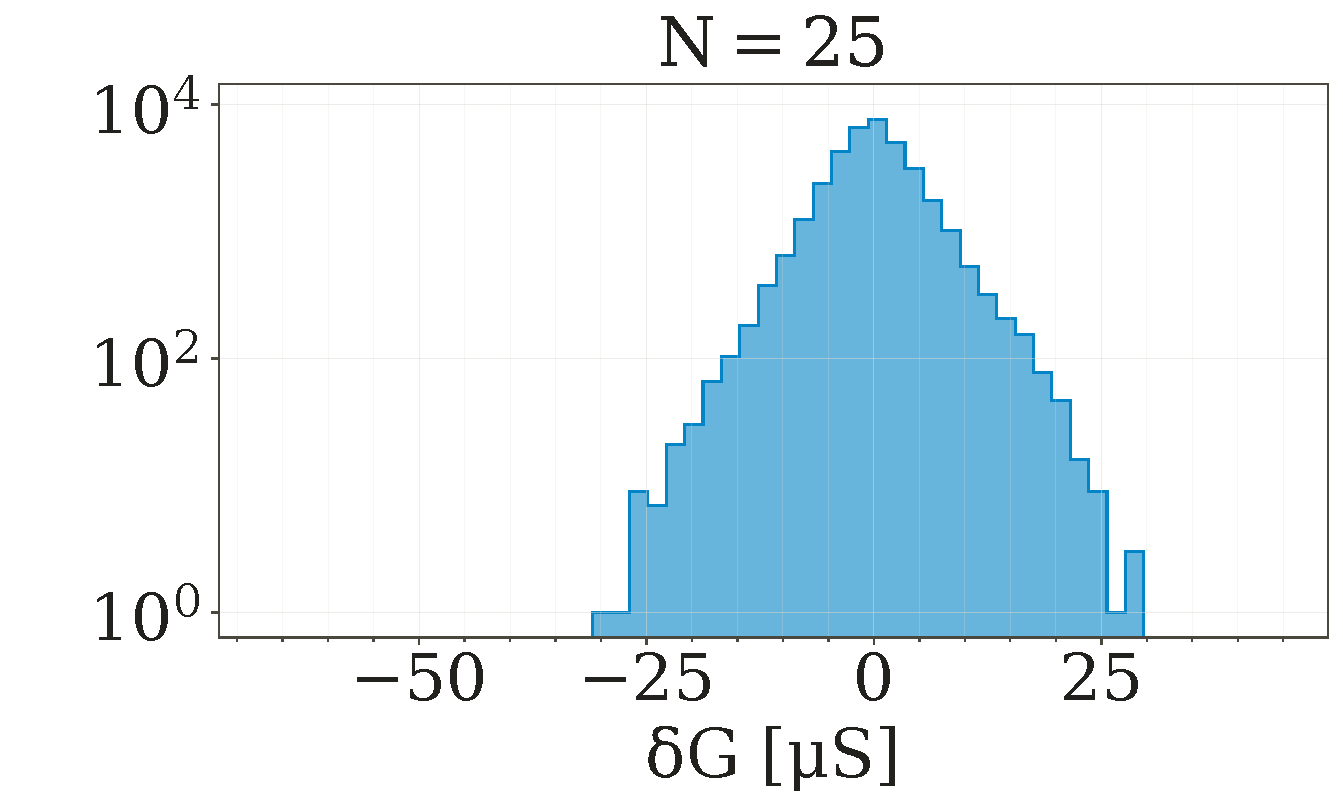
\includegraphics[width=0.68\linewidth]{figures/Histogram_25.pdf}\\[1pt]{\footnotesize $N=25$}
\end{minipage}\\[4pt]
\begin{minipage}[t]{0.47\linewidth}\centering
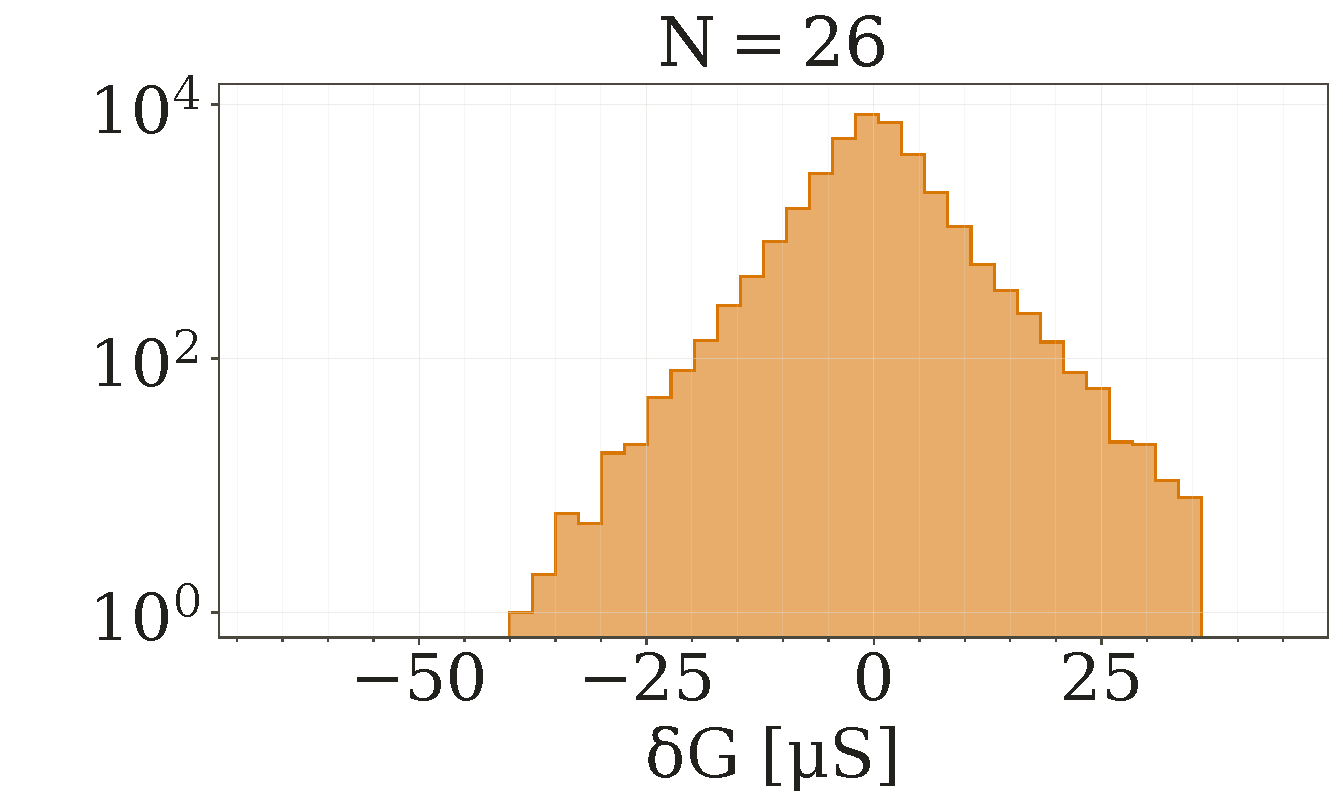
\includegraphics[width=0.68\linewidth]{figures/Histogram_26.pdf}\\[1pt]{\footnotesize $N=26$}
\end{minipage}%
\hfill
\begin{minipage}[t]{0.47\linewidth}\centering
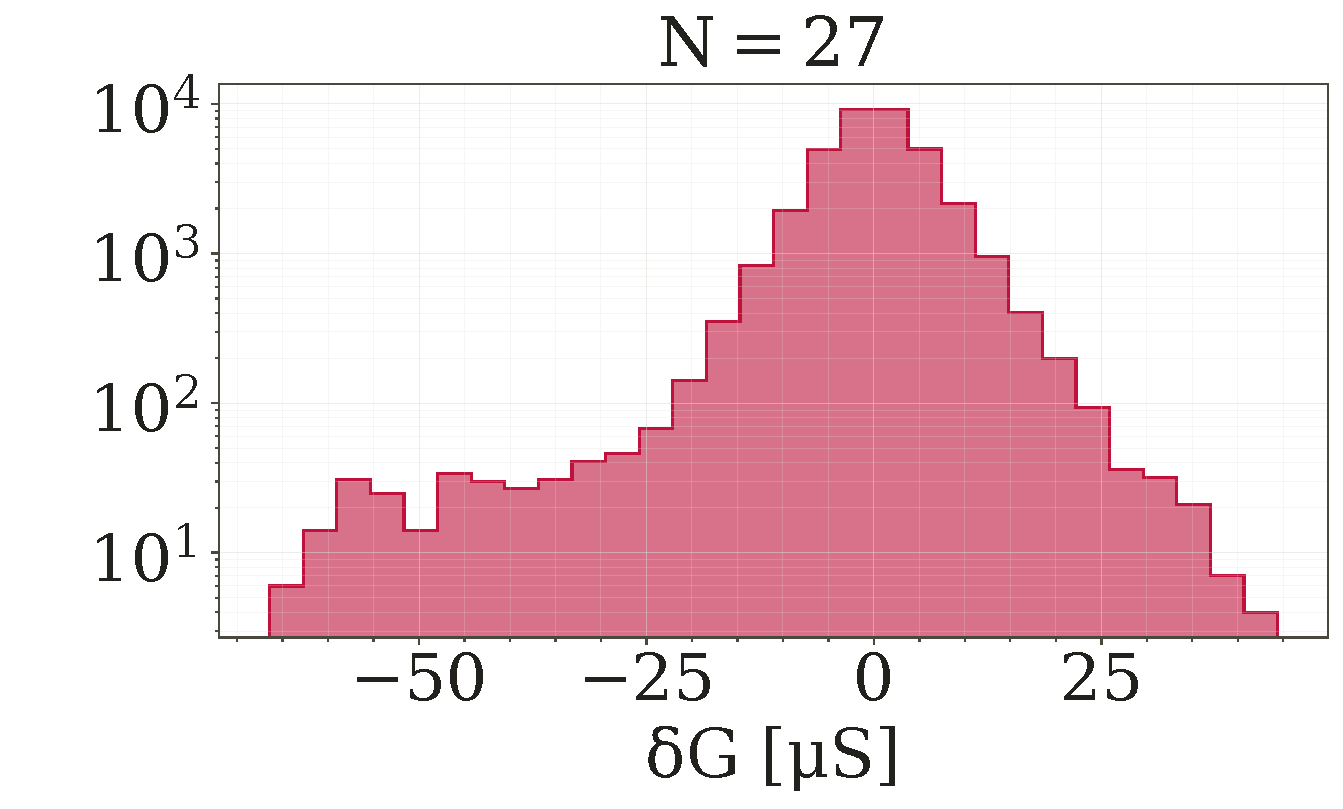
\includegraphics[width=0.68\linewidth]{figures/Histogram_27.pdf}\\[1pt]{\footnotesize $N=27$}
\end{minipage}
\end{center}
\smallskip
{\scriptsize $\delta G$ histograms ($\delta t = 2.5\,$s). $x=\delta G\,[\mu\text{S}]$, $y=$ counts (log). 50 bins, same for all 4 conditions.}
\smallskip

{\footnotesize\textbf{Key observations}
\begin{itemize}[itemsep=1pt,topsep=1pt,leftmargin=1em]
\item $\delta t = 2.5\,$s: point of maximal skewness for $N=27$.
\item Heavy, skewed tail at $N=27$ vs.\ near-symmetric $\varnothing$ and $N=25$.
\item Distribution width grows monotonically with $N$.
\end{itemize}}
\smallskip
\begin{center}
\begin{minipage}{\linewidth}\centering
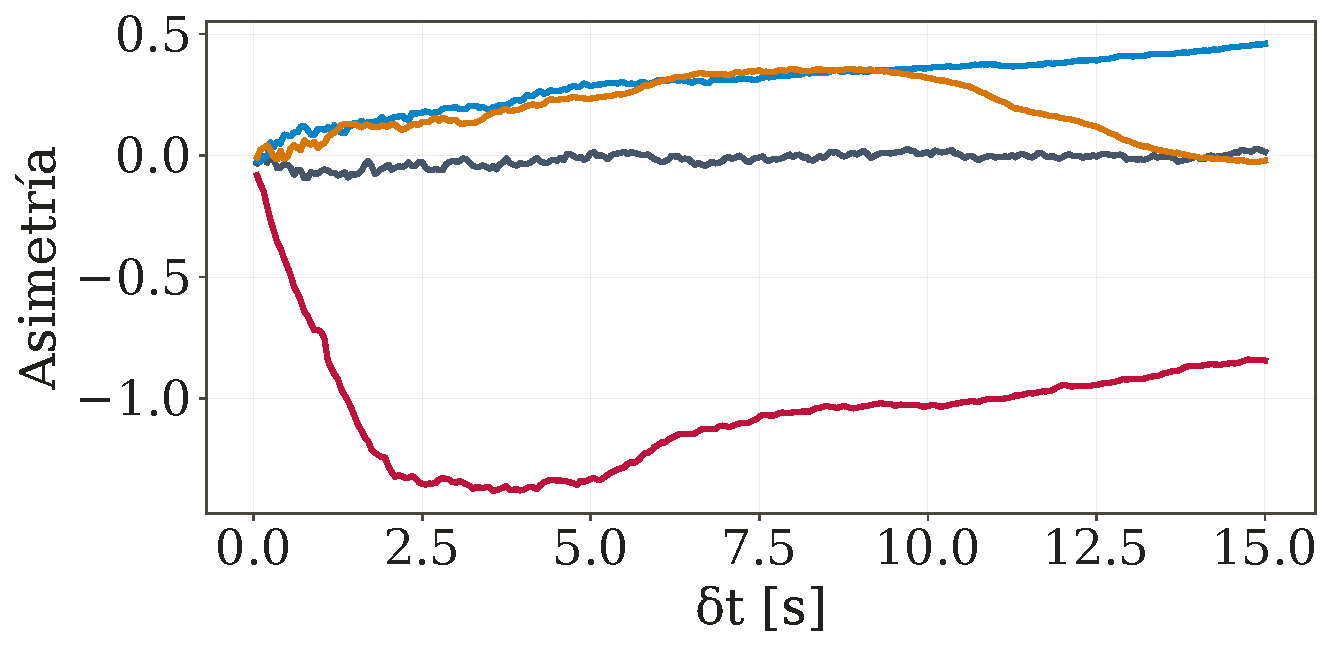
\includegraphics[width=0.60\linewidth]{figures/Skewness vs deltaT.pdf}
\end{minipage}
\end{center}
\smallskip
{\scriptsize Skewness of $\delta G$ over sliding windows of width $\delta t$, for each condition; its peak location sets the histogram window above.}
\end{posterbox}

\begin{posterbox}[name=dynamics,column=3,below=setupacq,bottomaligned=distributions,span=3]{{Dynamics \& Survival}}
\begin{center}
\begin{minipage}{\linewidth}\centering
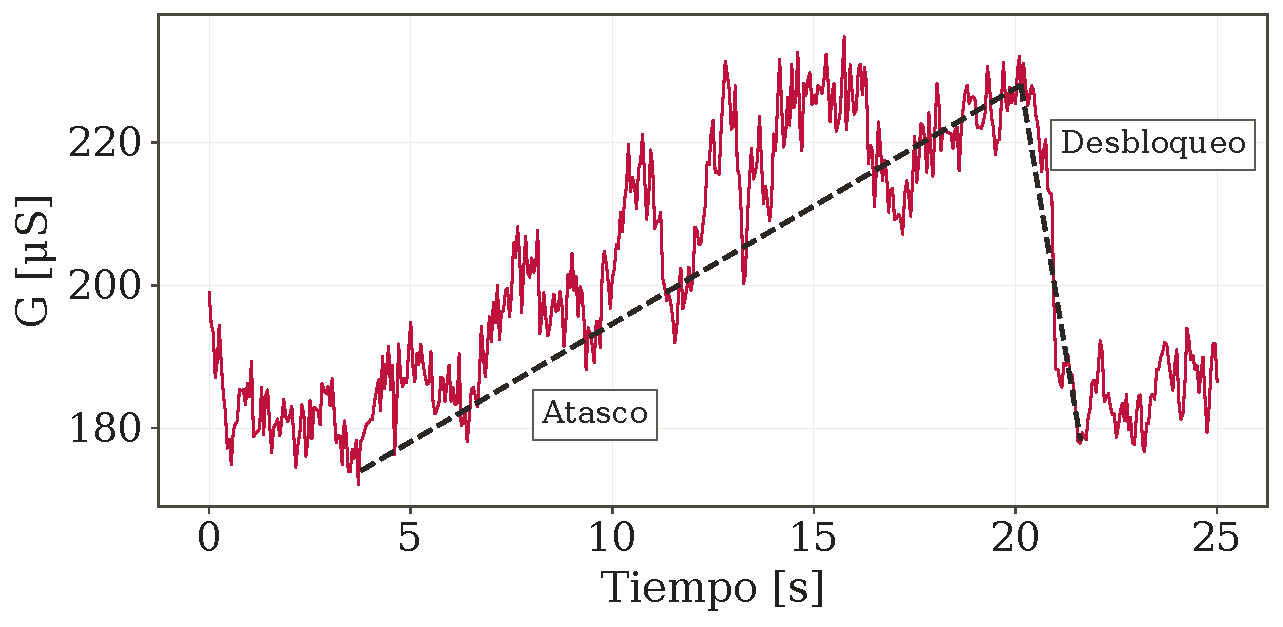
\includegraphics[width=0.60\linewidth]{figures/Jamming.pdf}
\end{minipage}
\end{center}
\smallskip
{\scriptsize Representative $G(t)$ segment around an unjamming event ($N=27$). The slow rise tracks pressure build-up as an arch blocks the exit; the sharp drop marks its collapse and the resumption of flow.}
\smallskip

{\footnotesize\textbf{Reading}
\begin{itemize}[itemsep=1pt,topsep=1pt,leftmargin=1em]
\item $\varnothing$: flat signal, sensor noise only.
\item $N=25$: moderate fluctuations, no extreme events.
\item $N=26$--$27$: large-amplitude jamming events.
\end{itemize}}
\smallskip
\begin{center}
\begin{minipage}{\linewidth}\centering
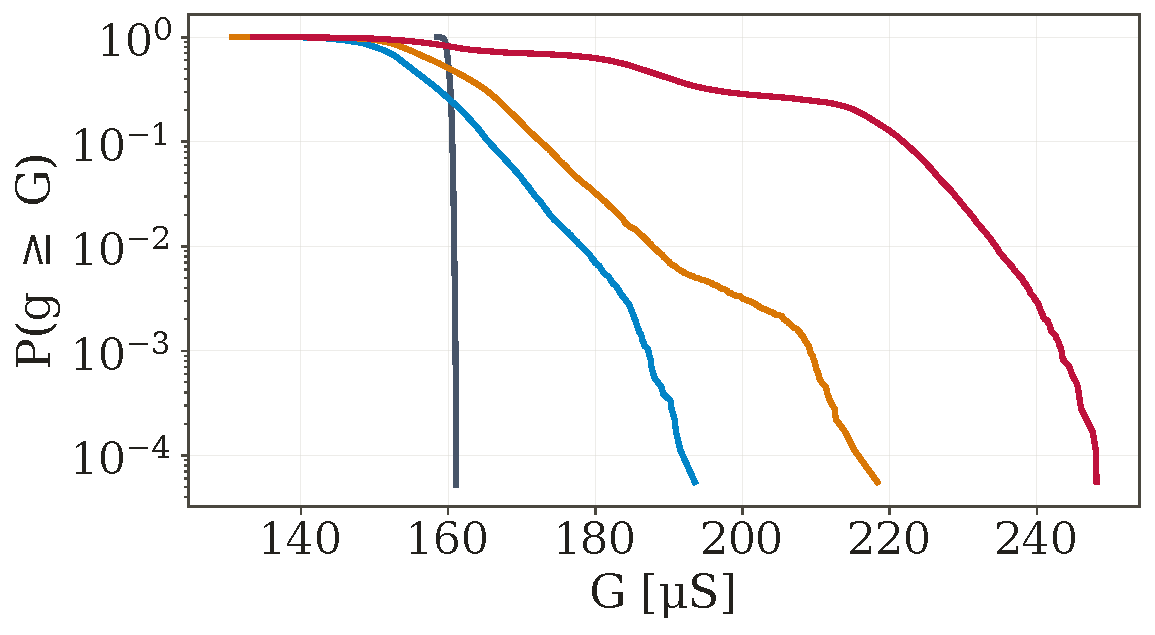
\includegraphics[width=0.60\linewidth]{figures/Supervivencia.pdf}
\end{minipage}
\end{center}
\smallskip
{\scriptsize Survival function. $x=G\,[\mu\text{S}]$, $y=P(G\ge g)$ (log scale). Same 4-condition color code throughout; the tail thickens with $N$.}
\end{posterbox}

%% ===========================================================================
%% ROW 4 -- Conclusions, Acknowledgements & References: ONE header, three
%% internal sub-columns via a tabular (see note 7). Uses below=distributions
%% + above=bottom so its frame always spans exactly from Row 3's bottom to
%% the physical page bottom, regardless of Row 3's final height.
%% ===========================================================================
\begin{posterbox}[name=conclusions,column=0,below=distributions,above=bottom,span=6]{{Conclusions, Acknowledgements \& References}}
\setlength{\tabcolsep}{0pt}
\small
\begin{tabular}{@{}p{0.315\linewidth}@{\hspace{0.02\linewidth}}p{0.315\linewidth}@{\hspace{0.02\linewidth}}p{0.315\linewidth}@{}}
% --- Column 1: Conclusions & Next Steps ---
{\bf Conclusions \& Next Steps}\par\smallskip
{\footnotesize
\begin{itemize}[itemsep=1.5pt,topsep=1pt,leftmargin=1em]
%\item Conductance fluctuations resolve free flow ($N=25$) from incipient congestion ($N=26$--$27$).
%\item $\delta G$ skewness and the tail of $G$'s survival function grow monotonically with density.
\item \textbf{Next:} deploy the distributed configuration to map spatial pressure inhomogeneities and correlate them with cluster dynamics.
\end{itemize}}
&
% --- Column 2: Acknowledgements ---
{\bf Acknowledgements}\par\smallskip
{\footnotesize Data color code used in every figure:}
\smallskip
\begin{center}
\footnotesize
\legendrow{cVacio}{$\varnothing$}\quad\legendrow{cN25}{$N{=}25$}\\[2pt]
\legendrow{cN26}{$N{=}26$}\quad\legendrow{cN27}{$N{=}27$}
\end{center}
\vspace{2pt}
\begin{center}

\includegraphics[height=1cm]{figures/logoITBA}\quad
\includegraphics[height=1cm]{figures/logoCONICET}
\end{center}
&
% --- Column 3: References ---
{\bf References}\par\smallskip
{\scriptsize
\begin{enumerate}[itemsep=1pt,topsep=1pt,leftmargin=1.3em]
\item[{[1]}] A.~P.~Solon \textit{et al.}, Nat. Phys. \textbf{11}, 673 (2015).
\item[{[2]}] G.~Junot \textit{et al.}, Phys. Rev. Lett. \textbf{119}, 028002 (2017).
\item[{[3]}] G.~A.~Patterson \textit{et al.}, Phys. Rev. Lett. \textbf{119}, 248301 (2017).
\item[{[4]}] M.~R.~Ferressini \textit{et al.}, Phys. Rev. E, 015406 (2025).
\item[{[5]}] R.~O.~Duda and P.~E.~Hart, Commun. ACM \textbf{15}, 11 (1972).
\end{enumerate}}
\\
\end{tabular}
\end{posterbox}

\end{poster}
\end{document}
